\begin{frame}
\frametitle{Signal region (SR) -- 2017 \mu\tauh\ channel as example}

\begin{block}{\mu\ and \tauh\ candidates}
\begin{minipage}{.5\linewidth}
\begin{itemize}
\item $L_1=\mu$
\begin{itemize}
\item $p_T > \SI{21}{\GeV}$, $\abs{\eta}<\num{2.1}$
\item $d_z < \SI{0.2}{\centi\meter}$, $d_{xy} < \SI{0.045}{\centi\meter}$
\item $\text{relative isolation} < \num{0.15}$
\item medium \texttt{muonID}
\end{itemize}
\item $L_2=\tauh$
\begin{itemize}
\item $p_T > \SI{30}{\GeV}$, $\abs{\eta}<\num{2.3}$
\item $d_z < \SI{0.2}{\centi\meter}$
\item $\text{relative isolation} < \num{0.15}$
\item NewDecayModeFinding (modes 5 to 9 vetoed)
\item deepTau anti-electron (VVL WP)
\item deepTau anti-muon (tight WP)
\item deepTau vs jet (medium WP)
\end{itemize}
\end{itemize}
\end{minipage}
\begin{minipage}{.49\linewidth}
\begin{center}
{\tdplotsetmaincoords{70}{115}
\tdplotsetrotatedcoords{-90}{-90}{-90}
\begin{tikzpicture}[tdplot_rotated_coords,scale=1]
%% base
\draw [->] (0,0,-3)--(0,0,3) node[above] {$\bvec_z$};
\draw [->] (0,0,0)--(1,0,0) node[above] {$\bvec_x$};
\draw [->] (0,0,0)--(0,1,0) node[above] {$\bvec_y$};

%% CMS barrel
\draw (0,0,-2.1) circle (1.5);
\draw (0,0,2.1) circle (1.5);
\def\CMSphiangle{70}
\draw ({1.5*cos(\CMSphiangle)},{1.5*sin(\CMSphiangle)},-2.1) --+(0,0,4.2);
\draw ({1.5*cos(180+\CMSphiangle)},{1.5*sin(180+\CMSphiangle)},-2.1) --+(0,0,4.2);

%% beam
\draw [ltcolorred, very thick, -latex] (0,0,-2)--(0,0,0);
\draw [ltcolorred, very thick, -latex] (0,0,2)--(0,0,0);
%% particule sortante
\draw [ltcolorblue, thick, -latex] (0,0,0)--(1.5,1.5,{1.5*2^0.5});
%% vertex primaire
\fill [ltcolororange] (0,0,0) circle (2pt);

%% track plane
\def\CMSphiangle{45}
\draw [densely dotted] ({1.5*cos(\CMSphiangle)},{1.5*sin(\CMSphiangle)},-2.1) -- ({1.5*cos(\CMSphiangle)},{1.5*sin(\CMSphiangle)},2.1) -- ({-1.5*cos(\CMSphiangle)},{-1.5*sin(\CMSphiangle)},2.1) -- ({-1.5*cos(\CMSphiangle)},{-1.5*sin(\CMSphiangle)},-2.1) --({1.5*cos(\CMSphiangle)},{1.5*sin(\CMSphiangle)},-2.1);

%% phi angle
\draw [densely dotted] (0,0,2.1)--(1.5,0,2.1);
\draw [-latex] (1,0,2.1) arc (0:45:1);
\draw (.75,.25,2.1) node {$\phi$};

%% theta angle
\tdplotsetrotatedcoords{0}{45}{90}
%\draw [tdplot_rotated_coords, ltcolorgreen,<->] (-2.1,1.5,0)--(2.1,-1.5,0);
%\draw [tdplot_rotated_coords, ltcolorgreen,<->] (-2.1,-1.5,0)--(2.1,1.5,0);
%\draw [tdplot_rotated_coords, ltcolorcyan,<->] (-1.5,2.1,0)--(1.5,-2.1,0);
%\draw [tdplot_rotated_coords, ltcolorcyan,<->] (-1.5,-2.1,0)--(1.5,2.1,0);
\draw [tdplot_rotated_coords,-latex] (1,0,0) arc (0:45:1);
\draw [tdplot_rotated_coords] (22.5:1.2) node {$\theta$};
\end{tikzpicture}}
\begin{equation*}
\eta = -\ln\tan\frac{\theta}{2}
\end{equation*}
\end{center}
\end{minipage}
\end{block}

\end{frame}

\begin{frame}
\frametitle{Values of $\eta$ and trajectories in CMS}
\begin{center}
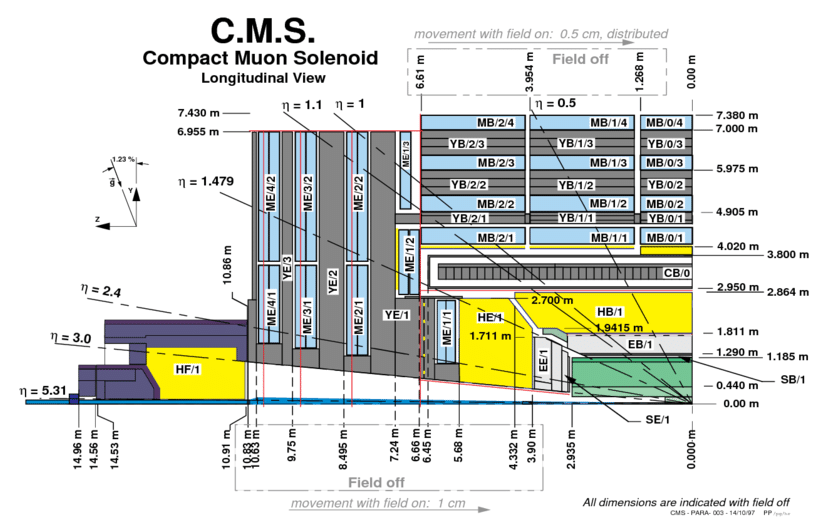
\includegraphics[width=\graphw, height=\graphh, keepaspectratio]{\PhDthesisdir/plots_and_images/from_CMS_alignment_photodetectors/CMS-eta-ranges.png}
\end{center}
\vspace{-9pt}
\end{frame}

\begin{frame}
\frametitle{Avoiding misidentification: Particles isolation -- qualitatively}
\begin{center}
\begin{tikzpicture}
\def\trackerrin{.100}
\def\trackerrout{1.185}
\def\trackercolor{ltcolorgray1}

\def\ECALrin{1.290}
\def\ECALrout{1.811}
\def\ECALcolor{ltcolorgreen1}

\def\HCALrin{1.812}
\def\HCALrout{2.854}
\def\HCALcolor{ltcoloryellow3}

\def\Solenrin{2.950}
\def\Solenrout{3.800}
\def\Solencolor{ltcolorgray2}

\def\ironryrina{3.850}
\def\ironryrouta{4.000}
\def\muonrina{4.020}
\def\muonrouta{4.400}
\def\ironryrinb{4.420}
\def\ironryroutb{4.880}
\def\muonrinb{4.905}
\def\muonroutb{5.285}
\def\ironryrinc{5.300}
\def\ironryroutc{5.960}
\def\muonrinc{5.975}
\def\muonroutc{6.355}
\def\ironryrind{6.375}
\def\ironryroutd{6.980}
\def\muonrind{7.000}
\def\muonroutd{7.380}
\def\muoncolor{ltcoloryellow1}
\def\ironrycolor{ltcolorred3}

\clip (-\graphw/2,-\graphh/2) rectangle (\graphw/2,\graphh/2);

\draw (0,0) coordinate (PV);

\foreach \rin/\rout/\color in {
\muonrind/\muonroutd/\muoncolor,
\ironryrind/\ironryroutd/\ironrycolor,
\muonrinc/\muonroutc/\muoncolor,
\ironryrinc/\ironryroutc/\ironrycolor,
\muonrinb/\muonroutb/\muoncolor,
\ironryrinb/\ironryroutb/\ironrycolor,
\muonrina/\muonrouta/\muoncolor,
%\ironryrina/\ironryrouta/\ironrycolor,
\Solenrin/\Solenrout/\Solencolor,
\HCALrin/\HCALrout/\HCALcolor,
\ECALrin/\ECALrout/\ECALcolor,
\trackerrin/\trackerrout/\trackercolor
}{
\fill (PV) [color = \color] circle (\rout);
\fill (PV) [color = white] circle (\rin);
}

\foreach \phiangle/\maxradius/\linecolor/\linethick in {
150/\HCALrin/ltcolorgreen/thin,
120/\HCALrin/ltcolorred/very thick,
122/\HCALrin/ltcolorred/thin,
117/\HCALrin/ltcolorred/thin,
0/\HCALrin/ltcolorblue/very thick,
5/\ECALrin/ltcolorblue/thin,
10/\HCALrin/ltcolorblue/thin,
-7/\ECALrin/ltcolorblue/thin,
-13/\HCALrin/ltcolorblue/thin,
8/\ECALrin/ltcolorblue/thin,
-2/\HCALrin/ltcolorblue/thin,
3/\ECALrin/ltcolorblue/thin}{
\draw [\linecolor, \linethick] (PV) --+ (\phiangle:\trackerrout);
\def\newmaxradius{\maxradius+.25}
\ifthenelse{\equal{\maxradius}{\ECALrin}}{\def\newmaxradius{\ECALrout}}{}
\ifthenelse{\equal{\maxradius}{\HCALrin}}{\def\newmaxradius{\HCALrout}}{}
\draw [\linecolor4, ultra thick] (PV)+(\phiangle:\maxradius)--+(\phiangle:\newmaxradius);
}

\end{tikzpicture}
\end{center}
\end{frame}

%\begin{frame}\addtocounter{framenumber}{-1}
%\frametitle{Particles isolation -- quantitatively}
%\begin{block}{}
%\begin{equation*}
%I_\text{rel}^{(\ell)}
=
\left.
\frac{1}{p_T^{(\ell)}}
\left[
\sum_{\hadron^\pm,\text{PV}} p_T^{\hadron^\pm}
+
\max\left(
0
,
\sum_{\hadron^0}p_{\hadron^0}
+
\sum_{\gamma}p_{\gamma}
- \Delta\beta
\sum_{\hadron^\pm,\text{PU}} p_T^{\hadron^\pm}
\right)
\right]
\right|_{\Delta R < R_\ell}
%\end{equation*}
%\begin{center}
%with $\Delta R = \sqrt{\Delta\phi^2+\Delta\eta^2}$.
%\end{center}
%\end{block}
%\pause
%\begin{block}{Particles isolation cut for SR}
%\begin{itemize}
%\item[$\ell$] $I_\text{rel}<\num{0.3}$,
%$R_\ell = \num{0.5}$.
%\item[\tauh] MVA-based isolation criterion with 3 available WP:
%\begin{itemize}
%\item Very Loose (VLoose),
%\item Medium,
%\item Tight (used for SR).
%\end{itemize}
%\end{itemize}
%\end{block}
%\end{frame}

\begin{frame}
\frametitle{Signal region (SR) -- 2017 \mu\tauh\ channel as example}

\begin{block}{Obtaining dileptons candidates}
\begin{minipage}[c]{.55\linewidth}
With all $L_1$ and $L_2$ passing selection,\\
compose  pairs ($L_1L_2$) respecting:
\begin{itemize}
\item opposed electric charges:\\ the initial Higgs is \textbf{neutral}.
\item pair separation $\Delta R > \num{0.5}$:\\ avoid fake dileptons from jet particles.
\end{itemize}
\end{minipage}
\begin{minipage}[c]{.4\linewidth}
\vspace{\baselineskip}
\begin{fmffile}{H-tautau_small}\fmfstraight
\begin{fmfchar*}(40,30)
  \fmfleft{h}
  \fmfright{tau1,tau2}
  \fmf{dashes, label=$\Hs,, \Hn,, \Ha$, l.side=left}{h,v}
  \fmf{fermion, label=$\tau^+$, l.side=left}{tau1,v}
  \fmf{fermion, label=$\tau^-$, l.side=left}{v,tau2}
  \fmfdot{v}
\end{fmfchar*}
\end{fmffile}
\vspace{\baselineskip}
\end{minipage}
\end{block}
\pause
\begin{block}{Selecting one dilepton}
Choose by:\\
~\hfill
most isolated $L_1$,
\hfill
highest $\pT^{L_1}$,
\hfill
most isolated $L_2$,
\hfill
highest $\pT^{L_2}$.
\hfill~
\end{block}

\end{frame}


\begin{frame}
\frametitle{Signal region (SR) -- 2017 \mu\tauh\ channel as example}

\begin{block}{Extra leptons: reject events containing}
\begin{itemize}
\item electron with $\pT > \SI{10}{\GeV}$, $\abs{\eta} < \num{2.4}$, \SI{90}{\%} eff. WP of the \texttt{electronID} MVA, $\text{rel. iso}<\num{0.3}$
\item second muon with $\pT > \SI{10}{\GeV}$, $\abs{\eta} < \num{2.4}$, medium \texttt{muonID}, $\text{rel. iso}<\num{0.3}$
\item opposite-charge muon pair ($\mu\mu$ channel overlapping)
\end{itemize}
\end{block}

\pause
\begin{block}{Transverse mass}
\begin{equation*}
m_T^{(\ell)}<\SI{70}{\GeV}
\msep
m_T^{(\ell)} = \sqrt{2p_T^{(\ell)} E_T^\text{miss}(1-\cos\Delta\phi)}
\end{equation*}
\end{block}
\end{frame}
